\section{Universal-Region Optimality and Deployment Extensions}

\subsection{A matching certification lower bound}

Consider two equally likely sources. Source zero emits
$\operatorname{Ber}(1/2)$ and source one emits
$\operatorname{Ber}(1/2+\theta)$. Their normalized Bayes source advantage is
exactly $\theta$.

\begin{theorem}[Binary embedded lower bound]
Fix a contract $\tau$, margin $\gamma$, soundness error $\delta$, and power
error $\beta$, where
$0<\gamma<\min\{\tau,1/2-\tau\}$ and $\delta+\beta<1/2$.
Any procedure that certifies $\theta=\tau-\gamma$ with probability at least
$1-\beta$ and certifies $\theta=\tau+\gamma$ with probability at most
$\delta$ requires
\begin{equation}
n\geq
\frac{\log(1/[2(\delta+\beta)])}
{\operatorname{KL}(\operatorname{Ber}(1/2+\tau-\gamma)
\Vert\operatorname{Ber}(1/2+\tau+\gamma))}
\label{supp:eq:binary-lower}
\end{equation}
observations from the informative source stratum.
\end{theorem}

\begin{proof}
The certification decision is a test between the safe and unsafe
experiments. Its two errors sum to at most $\delta+\beta$. The
Bretagnolle--Huber testing inequality lower-bounds that sum by
$\frac12\exp[-n\operatorname{KL}(P_{\rm safe}\Vert P_{\rm unsafe})]$.
The other source has the same law under both experiments and contributes no
KL. Rearranging proves Eq.~\eqref{supp:eq:binary-lower}.
\end{proof}

For $\tau$ bounded away from $1/2$, this is
$\Omega(\log(1/(\delta+\beta))/\gamma^2)$. More generally, consider protocols
required to return a distribution-uniform $\ell_1$ region that remains valid
for every bounded functional selected after viewing the same $K$-category
table. The dual identity
$\|p-q\|_1=\max_{v\in\{-1,1\}^K}v^\top(p-q)$ reduces simultaneous support
control to unrestricted multinomial $\ell_1$ estimation. Standard multinomial
packing and the binary subexperiment above give
\begin{equation}
n=\Omega\!\left(
\frac{K+\log(1/\delta)}{\gamma^2}\right).
\end{equation}
The Weissman radius used by MOSAIC gives the matching upper rate. This
optimality statement concerns universal same-table regions; a test of one
fixed scalar functional can be easier.

\subsection{Exact residual support and the infinite-sample floor}

Fix one label, common transform $T$, reference laws $p_s$, release channel
$M$, and residual budget $\eta$, so
\[
q_s=(1-\eta)p_sT+\eta r_s,
\]
where each $r_s$ is unrestricted. For attacker assignment $a$, let
$v_{a,s}$ be its score on the fine alphabet and
$R_a(q)=G^{-1}\sum_s q_s^\top v_{a,s}$.

\begin{theorem}[Sharp residual floor]
For every fixed attacker assignment and task-loss vector $u$,
\begin{align}
\sup_{r_{1:G}}R_a(q)
&=\frac{1-\eta}{G}\sum_s p_s^\top Tv_{a,s}
 +\frac{\eta}{G}\sum_s\max_c v_{a,s}(c),\\
\sup_r q_s^\top u
&=(1-\eta)p_s^\top Tu+\eta\max_c u(c).
\end{align}
These terms persist at zero reference radius and no uniformly valid
certificate over the stated bridge class can make them smaller. If two
common released laws coincide and $M$ has binary Dobrushin coefficient
$\alpha$, the class contains source advantage exactly $\eta\alpha$.
\end{theorem}

\begin{proof}
Each objective is linear in every residual law, hence maximized at a simplex
vertex placing all mass on a highest-scoring fine token. Those vertices belong
to the registered bridge class and attain both displays. For the final claim,
choose source residuals on two channel rows attaining total variation
$\alpha$; their common component cancels and the residual contribution has
total variation $\eta\alpha$.
\end{proof}

This separates statistical uncertainty from declared shift breadth. Tighter
multinomial regions can reduce the first, but only a narrower bridge class or
a more contractive channel can reduce the second. A locked census recomputes
all 35 primary BiasBios and ACS releases in four modes: full, zero reference
radius, zero residual, and both zero. Residual shift exceeds sampling in all
35 jobs for both source and utility. Median source increments are $.1914$
versus $4.01\times10^{-8}$; median utility increments are $.1377$ versus
$8.26\times10^{-9}$. An independent replay cross-checks every frozen release
and all summary statistics.

\subsection{Bounded correlated sessions}

Let a source be associated with $r$ fine items
$C_{1:r}$ having an arbitrary joint source-conditional law. Registered
channels $M_i$ release $Z_i$, with independent mechanism randomness
conditional on the complete fine tuple. Define
\[
M_{[r]}(c_{1:r},z_{1:r})=\prod_{i=1}^r M_i(c_i,z_i).
\]

\begin{theorem}[Exact bounded-session reduction]
Applying the MOSAIC envelope to a simultaneous confidence region for the joint
fine-tuple law and channel $M_{[r]}$ gives an exact universal-attacker
certificate for the complete transcript. No independence assumption is made
on $C_{1:r}$.
\end{theorem}

\begin{proof}
Conditional on the tuple, the displayed product is exactly the transcript
law. Marginalizing the unknown joint fine law through this row-stochastic
matrix produces the attacker's experiment. The adaptive-envelope proof
requires only a finite source law and a row-stochastic channel, so it applies
unchanged.
\end{proof}

Write
$\alpha_i=\max_{c,c'}\operatorname{TV}(M_i(c,\cdot),M_i(c',\cdot))$.
Maximal coupling of each item channel gives the scalable bound
\begin{equation}
\alpha(M_{[r]})\leq1-\prod_{i=1}^r(1-\alpha_i).
\label{supp:eq:session-capacity}
\end{equation}
Indeed, the transcript differs only if at least one item coupling differs.
The coupling characterization of total variation proves
Eq.~\eqref{supp:eq:session-capacity}; the normalized Bayes source advantage
for any number of sources is no larger than the same quantity. Arbitrary
registered adaptive session mechanisms are also covered after compilation
into one conditional transcript channel.

\subsection{Anytime-valid recertification}

For categorical counts $N_n$ and a fixed Dirichlet mixing law $\pi$, define
\begin{equation}
E_n(p)=
\frac{\int\prod_jq_j^{N_{n,j}}\,\pi(dq)}
{\prod_jp_j^{N_{n,j}}}.
\end{equation}

\begin{theorem}[Dirichlet-mixture confidence sequence]
Under law $p$, $E_n(p)$ is a nonnegative martingale with initial value one.
Consequently
$\mathcal C_n(\delta)=\{p:E_n(p)<1/\delta\}$ contains the true law
simultaneously for every $n\geq0$ with probability at least $1-\delta$,
including at arbitrary stopping times.
\end{theorem}

\begin{proof}
For every fixed $q$, its likelihood ratio against $p$ is a nonnegative
martingale. Integrating against a fixed mixing law preserves that property.
Ville's inequality bounds
$\Pr_p(\sup_n E_n(p)\geq1/\delta)$ by $\delta$.
\end{proof}

For Dirichlet parameter $a$ and $\widehat p=N_n/n$,
\[
\log E_n(p)=\log E_n(\widehat p)+
n\operatorname{KL}(\widehat p\Vert p).
\]
This identity gives an exact KL confidence sequence; Pinsker's inequality
provides the implemented $\ell_1$ outer radius. Allocating $\delta$ across
registered strata yields one event covering every MOSAIC channel selected at
every recertification time.

\subsection{Continuous release classes}

Let $q:x\mapsto\Delta_L$ range over a registered class with a finite
$\varepsilon$-net of size $N$ in
$\sup_x\|q(x)-q_j(x)\|_1$. Coordinate Hoeffding bounds and two approximation
terms give, simultaneously for every same-table selected $q$,
\begin{equation}
\left\|\mathbb E q(X)-\frac1n\sum_{i=1}^nq(X_i)\right\|_1
\leq
L\sqrt{\frac{\log(2LN/\delta)}{2n}}+2\varepsilon.
\label{supp:eq:continuous-cover}
\end{equation}
Passing these output-law regions through the identity channel gives the
finite-output MOSAIC certificate without first exposing a hard fine token.
For all thresholds $q_t(x)=(\mathbf1\{x\leq t\},\mathbf1\{x>t\})$, DKW removes
the finite net:
\[
\sup_t\left\|\mathbb E q_t(X)-n^{-1}\sum_iq_t(X_i)\right\|_1
\leq2\sqrt{\frac{\log(2/\delta)}{2n}}.
\]
Thus a threshold may be selected from the same audit sample with no grid or
threshold-count correction.

\subsection{Token-dependent real-proxy calibration}

Let $R$ be an imputed source and allow
$Q_y(s,c,r)=\Pr(R=r\mid S=s,C=c,Y=y)$ to vary with the fine token. If
$x_y(s,c)$ is the latent joint law, the observed proxy-token law is the linear
image
$r_y(r,c)=\sum_sQ_y(s,c,r)x_y(s,c)$.

\begin{theorem}[Token-dependent proxy bridge]
Suppose simultaneous regions cover the observed $r_y$ and every calibrated
row $Q_y(s,c,\cdot)$. Replacing the proxy observation matrix by this
token-dependent tensor and enlarging the observed-law radius by the largest
calibrated row radius contains the true latent law. The sharp conditional
token bounds follow from the same Charnes--Cooper LPs; an empty calibration
cell yields maximal uncertainty and abstention.
\end{theorem}

\begin{proof}
Writing $A_Q$ for the induced linear map,
$\|(A_Q-A_{\widehat Q})x\|_1$ is bounded by the largest calibrated row error,
since it is a convex combination of row errors. The triangle inequality puts
$A_{\widehat Q}x$ in the enlarged observed region. Conditional extrema are
linear-fractional functions over this polytope, so the existing
Charnes--Cooper reduction is exact.
\end{proof}

\subsection{A sharp privacy--utility conflict}

For a balanced binary source, write
$\kappa=\Pr(Y\neq S)$ after fixing the registered identification of task and
source labels.

\begin{theorem}[Source--task conflict]
Every released observation and decoder with task error $e_Y$ and source
advantage at most $\tau$ satisfies
\[
e_Y\geq\max\{0,(1-\tau)/2-\kappa\}.
\]
The same bound applies to worst-label error, and it is sharp when $Y=S$.
\end{theorem}

\begin{proof}
Use the task decoder as a source decoder. Its source error is at most
$e_Y+\kappa$, so the Bayes source error is no larger. Source advantage is
therefore at least $1-2(e_Y+\kappa)$. Rearrangement proves the bound. For
$Y=S$, a binary symmetric channel with crossover $(1-\tau)/2$ attains
equality.
\end{proof}

\section{Path-to-Deployment Confirmations}

\subsection{Locked theory implementation study}

The extension implementation was locked before execution; the artifact
manifest records SHA-256 prefix \texttt{99ccc7534bd1d194} and the complete
digest.
Across 1,000 optional-stopping runs for each $K\in\{2,4,8\}$, anytime false
exclusion occurs in 5, 2, and 0 runs, respectively, below the registered
familywise $.05$ level. Five product-channel rows match exact enumeration, and
500 continuous-threshold selections satisfy Eq.~\eqref{supp:eq:continuous-cover}.
The audit independently reconstructs every check and reports pass.

\subsection{Natural image-origin shift}

The frozen CINIC-10 store contains 48,000 file-provenanced images from four
classes, equally allocated across CIFAR-10 and ImageNet origin and across
construction, reference, bridge, and diagnostic roles. ResNet-18 penultimate
features are fixed before the audit. Five pre-outcome seeds compare Identity
and official closed-form LEACE and release 5/5 interfaces without a diagnostic
violation. After that result, a disclosed sequential power extension locks 35
new seeds and reruns all 40 under a stricter 40-seed familywise allocation.
MOSAIC releases 40/40 with 0/40 violations. Selected certified worst error
ranges from $.141$ to $.213$; diagnostic source advantage ranges from $.016$
to $.038$. The released channel costs a median $.60$ balanced-accuracy points
relative to its selected four-token task interface.

\subsection{Supported multi-hospital pathology shift}

A pre-outcome Camelyon17 lock fixes 39,200 official WILDS patches, five seeds,
ImageNet-pretrained ResNet-18 penultimate features, a four-token to two-token
release, and $.35$ source plus five utility contracts. Centers 0 and 3--4 form
the two audited hospital sources; every train and validation source--label
stratum contains 7,000 and 2,800 patches, respectively. The study concerns
supported multi-hospital patient shift and does not claim transport to the
unsupported center-2 test hospital.

The original external feature store was unavailable, so an outcome-blind
recovery used local official metadata and a pinned public WILDS mirror. A
data-access-only amendment after an HTTP rate limit serialized the reads,
added bounded retry, and checkpointed each shard. It changed no selected image,
model, feature, seed, threshold, contract, bridge, or analysis. Every retrieved
label, center, patient, node, and coordinate matches the locked metadata.

MOSAIC releases 5/5 interfaces at every utility threshold from $.35$ through
$.49$. Worst certified source advantage is $.2521$--$.2662$, and certified
worst error is $.2571$--$.2848$. Untouched validation diagnostics have source
advantage $.0126$--$.0274$ and worst error $.0964$--$.1428$. Thus all five
releases satisfy the held-out contracts, as do all 500 stochastic operational
replays. The independent auditor verifies every feature-array digest, receipt,
and deterministic replay.

\begin{table}[t]
\centering
\scriptsize
\setlength{\tabcolsep}{3.5pt}
\begin{tabular}{rrrrrr}
\hline
Seed & Cert.\ src. & Cert.\ err. & Held-out src. & Held-out err. & Op.\ viol.\\
\hline
4301 & .2521 & .2571 & .0214 & .1405 & 0/100\\
4302 & .2662 & .2848 & .0126 & .0964 & 0/100\\
4303 & .2561 & .2628 & .0141 & .1428 & 0/100\\
4304 & .2568 & .2673 & .0274 & .1096 & 0/100\\
4305 & .2613 & .2672 & .0142 & .1298 & 0/100\\
\hline
\end{tabular}
\caption{Locked Camelyon17 multi-hospital confirmation at the stricter $.35$
utility contract. All five interfaces release.}
\label{supp:tab:camelyon-streamed}
\end{table}

\subsection{A real estimated proxy}

A locked ACSIncome follow-up trains a source imputer from geography,
birthplace, ancestry, Hispanic origin, language, nativity, and citizenship on
a disjoint partition; balanced accuracy is $.8413$. True-source calibration
data estimate a label- and token-dependent confusion tensor, while the target
certificate sees proxy labels. The follow-up adds simultaneous source-mass
intervals to the latent-law polytope and uses its exact $\ell_1$ Chebyshev
center. This constraint was developed on a disclosed earlier split that
abstained, then locked under seed 20270725 before the new diagnostic outcome.

At 19,566 and 39,133 calibration rows, maximum conditional radii $.5534$ and
$.4771$ force abstention. At 58,700 and 78,267 rows, radii $.4126$ and $.3669$
permit release. The primary full-data certificate bounds source advantage by
$.2175/.2790$ and worst error by $.3691$. The untouched diagnostic values are
$.0590$ and $.2769$, with released expected balanced accuracy $.7729$ versus
$.8144$ for the unedited task score. The auditor independently reruns the
optimizer, verifies all 28 checks, and accounts for the complete $.05$
familywise budget. ACS lacks surnames, so the experiment is not labeled BISG.

\subsection{Matched local differential privacy}

For every primary MOSAIC release in BiasBios and ACS, a matched baseline uses
the same four-token input, binary output, bridge class, radii, and $.40$
utility contract. Four-ary randomized response keeps the registered task bit
with probability $.675$, giving $\epsilon_{\rm LDP}=.7309$ and Dobrushin
coefficient $.35$, exactly the source-advantage threshold. We enumerate all
16 deterministic fine-token task maps before applying that fixed channel.

Randomized response meets the stronger input-local-DP guarantee, but releases
0/35 interfaces because its certified task error exceeds $.40$. MOSAIC
releases 35/35 under its narrower source-inference contract and has lower
certified error in every job. The median, minimum, and maximum error penalties
for randomized response are $.1554$, $.0939$, and $.1710$. The independent
audit verifies all 35 local-DP channels, all source receipts, and the complete
summary.

\subsection{A prospective natural direct-rule failure}

The original ACS geographic study used 2018 California reference data and
held-out 2018 target states. A later pandemic-panel analysis identified two
fixed public-coverage interfaces that direct certification released while
MOSAIC abstained. The pattern was discovered in 2021 and persisted in 2022.
Before accessing 2023, a lock fixed both channels, their task decoders, Florida
as target, the $.40$ utility threshold, the exact Census archive member and
checksum, and a familywise Hoeffding lower bound over eight strata.

Both interfaces violate the threshold empirically in 27,772 Florida rows.
For the TaCo interface at seed 1401, worst error is $.42453$ and the familywise
lower bound is $.40542$, confirming a contract violation. The R-LACE
interface has error $.40812$ and lower bound $.38900$, so it is an empirical
but not familywise-confirmed violation. MOSAIC had abstained on both 2018
decisions. A separate 52-check auditor reconstructs the 2018 reference
functionals, verifies the streamed 2023 archive hash, and recomputes every
bound. This is a prospective confirmation of a previously identified failure
mode, not a first-look discovery.

\begin{figure*}[t]
\centering
\includegraphics[width=\textwidth]{figures/figure6_mosaic_path9_evidence.pdf}
\caption{Audited deployment evidence. (a) Increasing true-source calibration
support shrinks the real-proxy uncertainty region; the two smaller folds
abstain and the two larger folds release. (b) Every matched local-DP channel
has higher certified task error than MOSAIC, and all 35 miss the $.40$
utility contract. (c) Two direct releases frozen before 2023 both exceed the
contract empirically; the TaCo lower bound also clears it familywise.
Vertical bars in (c) extend from the familywise lower bound to the empirical
error.}
\label{supp:fig:path9-evidence}
\end{figure*}

\subsection{Designer chart}

\begin{figure}[t]
\centering
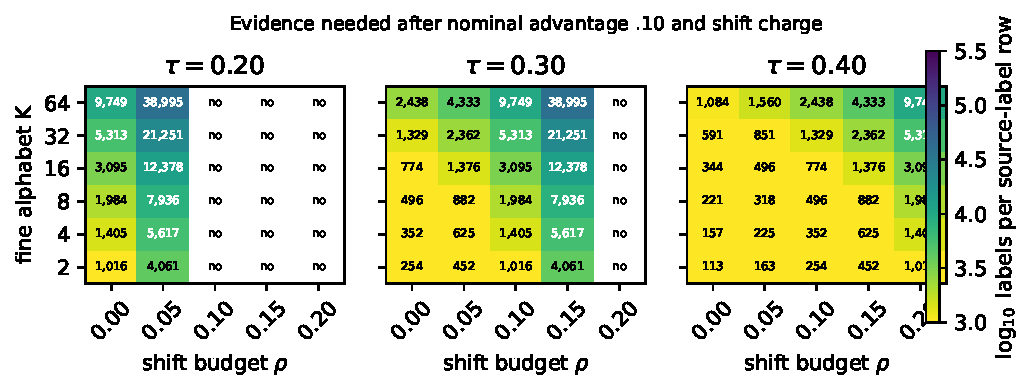
\includegraphics[width=.98\columnwidth]{mosaic_designer_chart_v1.pdf}
\caption{Sufficient labels per source--label stratum as a function of
alphabet size, source contract, and charged shift budget. Blank cells are
population-infeasible before sampling. The machine-readable chart contains
all 120 registered configurations.}
\label{supp:fig:designer-chart}
\end{figure}

For example, with four strata, nominal source advantage $.10$, contract
$\tau=.20$, and no shift charge, the sufficient counts are 1,016, 1,405, and
1,984 for $K=2,4,8$. A $.05$ shift charge reduces the statistical margin by
half and raises them to 4,061, 5,617, and 7,936. At shift charge $.10$, the
population bound already meets the contract and no finite sample can create
strict slack.

\subsection{Commensurate official FARE comparison}

Official FARE commit
\texttt{89cb1b66ed268c16} trains eight \texttt{fair\_gini\_eo} tree
representations on the same raw ACSIncome inputs and five-way partition as the
real-proxy study. Maximum leaves are $\{2,4\}$ and
$\alpha\in\{.80,.90,.95,.99\}$; every terminal leaf is judged by the same
token-dependent proxy calibration and $.35$ source, $.40$ task contracts.
All eight trees realize two leaves and abstain. Their worst source bound is
$1.0$ in one label and their worst conditional task bound is $1.0$; no
candidate is released and there is no false acceptance. This is an end-to-end
representation comparison under one commensurate release contract. It does
not reinterpret FARE's original demographic-parity theorem as a
source-inference guarantee.

\section{Mechanized Core and Auditor-Facing Tool}

The Lean 4 project under \texttt{research/formal/MosaicFormal} machine-checks
the adaptive-selection implication, familywise lifting, and the discrete
bridge residual construction used by Theorems 1--2. Its build receipt records
Lean 4.32.1 and theorem names
\texttt{adaptive\_exact\_envelope\_sound},
\texttt{adaptive\_family\_envelope\_sound},
\texttt{bridge\_residual\_reconstruct}, and
\texttt{adaptive\_bridge\_residual\_reconstruct}. Concentration inequalities,
LP duality, and floating-point solver correctness remain separately audited by
the 585-check implementation-independent replay.

The installable \texttt{mosaic-certified-release} package exposes
\texttt{fit}, \texttt{certify}, and \texttt{release\_or\_abstain}. The
\texttt{mosaic-audit} command validates a serialized certificate and emits a
versioned JSON or text report. Runtime monitoring records evidence age,
contract version, support state, and recertification decisions; failed or
expired evidence closes the release. A stand-alone replication packet specifies
exact commands, expected hashes, and discrepancy reporting for an evaluator
outside the project. No external replication is claimed in this submission.
